\section{中值定理与泰勒公式}

这一章有两组工具。中值定理把区间上的平均变化率与某一点的瞬时变化率联系起来；泰勒公式把函数在一点附近换成一个多项式，再加一个可以控制的余项。前者适合处理函数值的差、不等式放缩和方程根的个数，后者适合求极限、估计误差和判断高阶极值。

\subsection{极值点与罗尔定理}

先看一个熟悉的画面：一条光滑曲线在最高点或最低点处，切线是水平的。把这句话说精确，就是费马引理。

\begin{mydef}{局部极值}{calc4-local-extremum}
设 $f$ 在 $x_0$ 的某邻域内有定义。若存在 $\delta>0$，使得当 $|x-x_0|<\delta$ 时总有 $f(x)\le f(x_0)$，就称 $f$ 在 $x_0$ 取\textbf{局部极大值}；把不等号反向，得到\textbf{局部极小值}。极大值和极小值统称局部极值，$x_0$ 叫极值点。
\end{mydef}

注意定义只比较 $x_0$ 附近的值，不比较整个定义域。因此一个函数可以有很多个局部极值，局部极大值甚至可能小于另一个位置的局部极小值。

\begin{conclusion}{费马引理}{calc4-fermat}
若 $f$ 在 $x_0$ 取局部极值，且 $f$ 在 $x_0$ 可导，则 $f'(x_0)=0$。
\end{conclusion}

证明只用导数的定义。设 $x_0$ 是局部极大值点。当 $h>0$ 足够小时，$f(x_0+h)\le f(x_0)$，于是
\[
\frac{f(x_0+h)-f(x_0)}{h}\le 0.
\]
令 $h\to0^+$，右导数小于等于零。当 $h<0$ 时，分母为负，分子仍小于等于零，差商反而大于等于零；令 $h\to0^-$，左导数大于等于零。导数存在，左右导数都等于 $f'(x_0)$，所以 $f'(x_0)=0$。极小值的情形把不等号全部反过来即可。

反过来不成立。$f(x)=x^3$ 在 $x=0$ 处导数为零，但 $x<0$ 时 $f(x)<0$，$x>0$ 时 $f(x)>0$，$x=0$ 不是极值点。导数为零的点叫驻点，驻点只是极值的候选。费马引理也不能用在区间端点：端点只有单侧邻域，差商只有一个方向。

\begin{center}
\begin{tikzpicture}
\begin{axis}[width=0.78\linewidth, height=5.2cm,
  xlabel={$x$}, ylabel={$y$},
  xmin=-1.3, xmax=3.3, ymin=-3.2, ymax=3.2,
  xtick={-1,0,1,2,3}, ytick={-2,0,2},
  domain=-1.1:3.1, samples=160, font=\footnotesize]
\addplot[blue,thick] {x^3-3*x^2+2};
\draw[dashed,gray!70] (axis cs:-1.3,2) -- (axis cs:3.3,2);
\draw[dashed,gray!70] (axis cs:-1.3,-2) -- (axis cs:3.3,-2);
\addplot[only marks,mark=*,red!70!black] coordinates {(0,2)};
\addplot[only marks,mark=*,red!70!black] coordinates {(2,-2)};
\node[font=\scriptsize,anchor=south west] at (axis cs:0.05,2.05) {$f'(0)=0$};
\node[font=\scriptsize,blue!60!black,anchor=north west] at (axis cs:2.12,-2.24) {极小 $f'=0$};
\node[font=\scriptsize,blue!60!black,anchor=south] at (axis cs:-0.35,2.35) {极大};
\end{axis}
\end{tikzpicture}\\[2pt]
{\footnotesize 图 1：$f(x)=x^3-3x^2+2$ 在 $x=0$ 取极大值、在 $x=2$ 取极小值，两处切线都水平。反过来，驻点不一定极值，例如 $x^3$ 在 $0$ 处。}
\end{center}

把费马引理用在区间内部的最值点上，就得到罗尔定理。

\begin{conclusion}{罗尔定理}{calc4-rolle}
设 $f$ 在 $[a,b]$ 上连续，在 $(a,b)$ 内可导，且 $f(a)=f(b)$。则存在 $\xi\in(a,b)$，使 $f'(\xi)=0$。
\end{conclusion}

证明的思路是“最值点必在内部”。$f$ 在闭区间上连续，一定有最大值 $M$ 和最小值 $m$。若 $M=m$，$f$ 是常数，任取 $\xi\in(a,b)$ 都有 $f'(\xi)=0$。否则 $M,m$ 不可能都等于端点值 $f(a)=f(b)$，至少有一个最值在内部某点 $\xi$ 取到。这个 $\xi$ 是局部极值点，又在内点可导，费马引理给出 $f'(\xi)=0$。

定理只保证存在，不保证唯一。三个条件也不能省：$f(x)=x$ 在 $[0,1]$ 上连续可导，但 $f(0)\ne f(1)$，没有水平切线；$f(x)=|x|$ 在 $[-1,1]$ 上连续且 $f(-1)=f(1)$，但在 $x=0$ 不可导，曲线在原点出现尖角，仍然没有水平切线。

\begin{center}
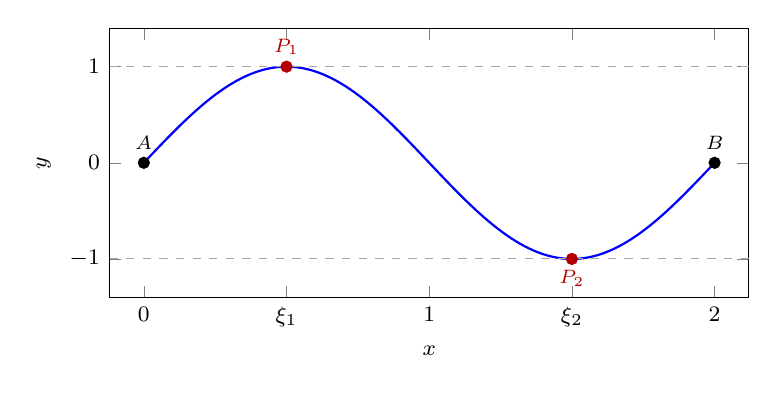
\begin{tikzpicture}
\begin{axis}[width=0.8\linewidth, height=5.0cm,
  xlabel={$x$}, ylabel={$y$},
  xmin=-0.12, xmax=2.12, ymin=-1.4, ymax=1.4,
  xtick={0,0.5,1,1.5,2},
  xticklabels={$0$,$\xi_1$,$1$,$\xi_2$,$2$},
  ytick={-1,0,1},
  domain=0:2, samples=200, font=\footnotesize]
\addplot[blue,thick] {sin(180*x)};
\draw[dashed,gray!70] (axis cs:-0.12,1) -- (axis cs:2.12,1);
\draw[dashed,gray!70] (axis cs:-0.12,-1) -- (axis cs:2.12,-1);
\addplot[only marks,mark=*] coordinates {(0,0)};
\addplot[only marks,mark=*] coordinates {(2,0)};
\addplot[only marks,mark=*,red!70!black] coordinates {(0.5,1)};
\addplot[only marks,mark=*,red!70!black] coordinates {(1.5,-1)};
\node[font=\scriptsize,anchor=south] at (axis cs:0,0.04) {$A$};
\node[font=\scriptsize,anchor=south] at (axis cs:2,0.04) {$B$};
\node[font=\scriptsize,red!70!black,anchor=south] at (axis cs:0.5,1.02) {$P_1$};
\node[font=\scriptsize,red!70!black,anchor=north] at (axis cs:1.5,-1.02) {$P_2$};
\end{axis}
\end{tikzpicture}\\[2pt]
{\footnotesize 图 2：端点 $A,B$ 等高时，曲线上至少有一处切线水平。图中 $P_1,P_2$ 两处都水平，说明定理中的 $\xi$ 可以不止一个。}
\end{center}

\subsection{拉格朗日与柯西中值定理}

罗尔定理要求两端等高。如果不等高，把函数减去连接端点的直线，就回到罗尔定理。具体地，令
\[
\varphi(x)=f(x)-f(a)-\frac{f(b)-f(a)}{b-a}(x-a).
\]
这个 $\varphi$ 在 $a,b$ 两点的值都是零：$\varphi(a)=f(a)-f(a)-0=0$，$\varphi(b)=f(b)-f(a)-[f(b)-f(a)]=0$。对 $\varphi$ 用罗尔定理，存在 $\xi\in(a,b)$ 使
\[
0=\varphi'(\xi)=f'(\xi)-\frac{f(b)-f(a)}{b-a},
\]
移项即得下面的定理。

\begin{conclusion}{拉格朗日中值定理}{calc4-lagrange}
设 $f$ 在 $[a,b]$ 上连续，在 $(a,b)$ 内可导。则存在 $\xi\in(a,b)$，使
\[
f(b)-f(a)=f'(\xi)(b-a).
\]
\end{conclusion}

等价的写法是 $f'(\xi)=\dfrac{f(b)-f(a)}{b-a}$：某点的切线斜率等于割线斜率。$\xi$ 的确切位置通常不知道，也不必知道；定理的用处是把函数值的差换成导数值。

把区间写成 $[x_0,x]$ 或 $[x,x+\Delta x]$，得到两种常用形式：
\[
f(x)=f(x_0)+f'(\xi)(x-x_0),\qquad \xi\text{ 在 }x_0\text{ 与 }x\text{ 之间},
\]
\[
f(x+\Delta x)-f(x)=f'(x+\theta\Delta x)\,\Delta x,\qquad 0<\theta<1.
\]
第二式叫有限增量公式。自变量走一步 $\Delta x$，函数走的那一步等于区间内某点的导数乘 $\Delta x$。它说明可导函数的增量可以被某个瞬时变化率代表。

由拉格朗日定理可以直接得到几个常用结论。若 $f'\equiv0$，则 $f$ 为常数：任取 $x_1<x_2$，有 $f(x_2)-f(x_1)=f'(\xi)(x_2-x_1)=0$。若 $f'\ge0$，则 $f$ 单调不减；若 $f'>0$，则 $f$ 严格递增。若两个函数导数处处相等，则它们相差一个常数。这些结论在不等式和零点问题里会反复用到。

\begin{center}
\begin{tikzpicture}
\begin{axis}[width=0.8\linewidth, height=5.4cm,
  xlabel={$x$}, ylabel={$y$},
  xmin=-0.2, xmax=3.3, ymin=-0.55, ymax=5.0,
  xtick={0,1,2,3}, ytick={0,1,2,3,4},
  domain=0:3, samples=160, font=\footnotesize]
\addplot[blue,thick] {x^2/2};
\addplot[gray!70,thick] {1.5*x};
\addplot[red!70!black,thick,dashed] {1.5*x-1.125};
\draw[gray!60,dashed] (axis cs:3,0) -- (axis cs:3,4.5);
\node[font=\scriptsize,anchor=south] at (axis cs:1.5,0.02) {$b-a$};
\node[font=\scriptsize,rotate=90] at (axis cs:3.14,2.25) {$f(b)-f(a)$};
\node[font=\scriptsize,gray!60!black] at (axis cs:2.55,4.05) {割线 $AB$};
\node[font=\scriptsize,red!70!black] at (axis cs:2.35,2.45) {切线};
\addplot[only marks,mark=*] coordinates {(0,0)};
\addplot[only marks,mark=*] coordinates {(3,4.5)};
\addplot[only marks,mark=*,red!70!black] coordinates {(1.5,1.125)};
\node[font=\scriptsize,anchor=north west] at (axis cs:0.03,0.06) {$A$};
\node[font=\scriptsize,anchor=south east] at (axis cs:2.97,4.52) {$B$};
\node[font=\scriptsize,red!70!black,anchor=south east] at (axis cs:1.38,1.45) {$P(\xi,f(\xi))$};
\end{axis}
\end{tikzpicture}\\[2pt]
{\footnotesize 图 3：割线 $AB$ 的斜率是 $\dfrac{f(b)-f(a)}{b-a}$。把割线平移，总会与曲线相切于某点 $P$，该点切线平行于 $AB$，这就是 $f'(\xi)(b-a)=f(b)-f(a)$。}
\end{center}

拉格朗日定理比较的是一个函数的增量与自变量的增量。如果把自变量也换成另一个函数 $g$，比较两个函数的增量比，就得到柯西中值定理。

\begin{conclusion}{柯西中值定理}{calc4-cauchy}
设 $f,g$ 在 $[a,b]$ 上连续，在 $(a,b)$ 内可导，且对一切 $x\in(a,b)$，$g'(x)\ne0$。则存在 $\xi\in(a,b)$，使
\[
\frac{f(b)-f(a)}{g(b)-g(a)}=\frac{f'(\xi)}{g'(\xi)}.
\]
\end{conclusion}

条件 $g'\ne0$ 有两个作用。第一，保证 $g(b)-g(a)\ne0$：如果 $g(b)=g(a)$，罗尔定理会给出某个 $g'=0$，与条件矛盾，所以分母有意义。第二，在参数曲线 $(g(t),f(t))$ 上，$g'\ne0$ 保证曲线没有竖直切线，切线斜率 $f'/g'$ 才有定义。

证明与拉格朗日定理类似。令
\[
F(x)=[f(b)-f(a)]g(x)-[g(b)-g(a)]f(x).
\]
直接计算得 $F(a)=F(b)=f(b)g(a)-g(b)f(a)$。由罗尔定理，存在 $\xi\in(a,b)$ 使 $F'(\xi)=0$，即
\[
[f(b)-f(a)]g'(\xi)-[g(b)-g(a)]f'(\xi)=0,
\]
整理就是柯西中值定理。取 $g(x)=x$，它就退化为拉格朗日定理。柯西定理也是证明洛必达法则和带拉格朗日余项的泰勒公式的工具。

\begin{center}
\begin{tikzpicture}
\begin{axis}[width=0.8\linewidth, height=5.4cm,
  xlabel={$x=g(t)$}, ylabel={$y=f(t)$},
  xmin=-0.2, xmax=4.3, ymin=-0.4, ymax=8.5,
  xtick={0,1,2,3,4}, ytick={0,2,4,6,8},
  font=\footnotesize, legend pos=south east,
  legend style={font=\scriptsize}]
\addplot[blue,thick, variable=t, domain=0.5:2, samples=120] ({t^2},{t^3});
\addlegendentry{曲线 $(g(t),f(t))$}
\addplot[gray!70,thick, domain=0:4.2] {2.1*x-0.4};
\addlegendentry{割线 $AB$}
\addplot[red!70!black,thick,dashed, domain=0:4.2] {2.1*x-1.372};
\addlegendentry{切线}
\addplot[only marks,mark=*] coordinates {(0.25,0.125)};
\addplot[only marks,mark=*] coordinates {(4,8)};
\addplot[only marks,mark=*,red!70!black] coordinates {(1.96,2.744)};
\node[font=\scriptsize,anchor=west] at (axis cs:0.36,0.62) {$A$};
\node[font=\scriptsize,anchor=west] at (axis cs:4.06,7.82) {$B$};
\node[font=\scriptsize,red!70!black,anchor=north west] at (axis cs:1.98,2.66) {$P$};
\end{axis}
\end{tikzpicture}\\[2pt]
{\footnotesize 图 4：把 $(g(t),f(t))$ 看成平面曲线，弦 $AB$ 的斜率是 $\dfrac{\Delta f}{\Delta g}$。柯西定理说，曲线上某点 $P$ 的切向量 $(g'(\xi),f'(\xi))$ 与弦平行，所以两个斜率相等。}
\end{center}
\subsection{用中值定理处理不等式与零点}

中值定理本身很短，难的是怎么用。下面两类问题最常见：证明不等式，判断方程根的个数。

\paragraph{不等式.} 第一条路是移项构造函数，用导数判断单调性。比如要证 $x>0$ 时 $e^x>1+x$，令 $F(x)=e^x-1-x$。则 $F'(x)=e^x-1$，在 $x>0$ 时为正，而 $F(0)=0$，所以 $F(x)>0$。$x<0$ 时 $F'<0$，$F$ 随 $x$ 增大而减小，从左侧靠近 $0$ 仍有 $F(x)>F(0)=0$。因此 $e^x\ge1+x$ 对一切实数成立，只在 $x=0$ 取等号。

第二条路是把函数值的差写成 $f'(\xi)(b-a)$，再对 $f'(\xi)$ 放缩。例如对任意实数 $x,y$，在 $x,y$ 之间用拉格朗日定理：
\[
\sin x-\sin y=\cos\xi\,(x-y),
\]
取绝对值，
\[
|\sin x-\sin y|=|\cos\xi|\,|x-y|\le |x-y|.
\]
这里的关键是 $|\cos\xi|\le1$ 有统一上界。如果导数在区间上无界，这条路的放缩就失效，需要换方法。

\begin{center}
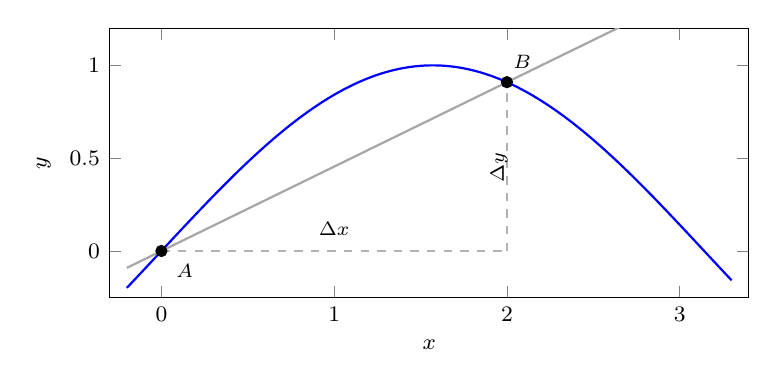
\begin{tikzpicture}
\begin{axis}[width=0.8\linewidth, height=5.0cm,
  xlabel={$x$}, ylabel={$y$},
  xmin=-0.3, xmax=3.4, ymin=-0.25, ymax=1.2,
  xtick={0,1,2,3}, ytick={0,0.5,1},
  domain=-0.2:3.3, samples=200, font=\footnotesize]
\addplot[blue,thick] {sin(deg(x))};
\addplot[gray!70,thick] {0.4546*x};
\draw[gray!60,dashed] (axis cs:2,0) -- (axis cs:2,0.9093);
\draw[gray!60,dashed] (axis cs:0,0) -- (axis cs:2,0);
\addplot[only marks,mark=*] coordinates {(0,0)};
\addplot[only marks,mark=*] coordinates {(2,0.9093)};
\node[font=\scriptsize,anchor=north west] at (axis cs:0.03,-0.02) {$A$};
\node[font=\scriptsize,anchor=south west] at (axis cs:1.98,0.93) {$B$};
\node[font=\scriptsize,anchor=south] at (axis cs:1.0,0.03) {$\Delta x$};
\node[font=\scriptsize,rotate=90,anchor=south] at (axis cs:2.06,0.45) {$\Delta y$};
\end{axis}
\end{tikzpicture}\\[2pt]
{\footnotesize 图 5：弦 $AB$ 的斜率是 $\cos\xi$。因为 $|\cos\xi|\le1$，竖直方向的差 $|\Delta y|$ 不超过水平方向的差 $|\Delta x|$。}
\end{center}

\paragraph{零点.} 判断方程 $f(x)=0$ 的根，先解决“有没有”，再解决“有几个”。

存在性靠零点定理：若 $f$ 在 $[a,b]$ 上连续，且 $f(a)f(b)<0$，则 $(a,b)$ 内至少有一个根。个数靠罗尔定理：若 $f$ 有 $n+1$ 个零点 $x_0<x_1<\cdots<x_n$，则在每个小区间 $(x_i,x_{i+1})$ 内都存在 $\xi_i$ 使 $f'(\xi_i)=0$。也就是说，$f$ 的 $n+1$ 个零点逼出了 $f'$ 的至少 $n$ 个零点。反过来，若 $f'$ 在区间内只有 $k$ 个零点，则 $f$ 至多有 $k+1$ 个零点。

定位则靠单调性。$f'$ 的零点把定义域分成若干段，每段上 $f$ 单调，因而每段至多一个根。把零点定理用在这些段上，就能判断哪一段真的有根。

看一个例子：
\[
f(x)=x^3-3x^2+2x=x(x-1)(x-2).
\]
它的三个根 $0,1,2$ 一眼能看出，重点是看导数怎样把根隔开。求导得
\[
f'(x)=3x^2-6x+2,
\]
两个零点为 $1\pm\dfrac{\sqrt3}{3}$，约等于 $0.423$ 和 $1.577$。它们分别落在 $(0,1)$ 和 $(1,2)$ 内，正好是罗尔定理在两个相邻根之间给出的点。另一方面，$f'$ 只有两个零点，所以 $f$ 不可能有第四个根。

\begin{center}
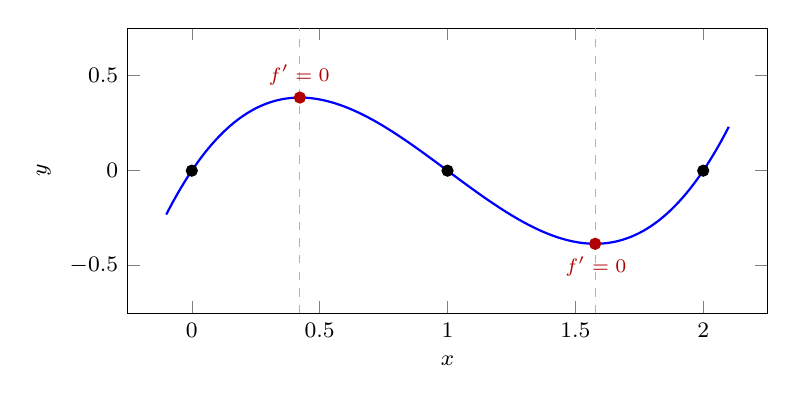
\begin{tikzpicture}
\begin{axis}[width=0.8\linewidth, height=5.2cm,
  xlabel={$x$}, ylabel={$y$},
  xmin=-0.25, xmax=2.25, ymin=-0.75, ymax=0.75,
  xtick={0,0.5,1,1.5,2}, ytick={-0.5,0,0.5},
  domain=-0.1:2.1, samples=160, font=\footnotesize]
\addplot[blue,thick] {x^3-3*x^2+2*x};
\draw[dashed,gray!60] (axis cs:0.4226,-0.75) -- (axis cs:0.4226,0.75);
\draw[dashed,gray!60] (axis cs:1.5774,-0.75) -- (axis cs:1.5774,0.75);
\addplot[only marks,mark=*] coordinates {(0,0)};
\addplot[only marks,mark=*] coordinates {(1,0)};
\addplot[only marks,mark=*] coordinates {(2,0)};
\addplot[only marks,mark=*,red!70!black] coordinates {(0.4226,0.3849)};
\addplot[only marks,mark=*,red!70!black] coordinates {(1.5774,-0.3849)};
\node[font=\scriptsize,red!70!black,anchor=south] at (axis cs:0.42,0.40) {$f'=0$};
\node[font=\scriptsize,red!70!black,anchor=north] at (axis cs:1.58,-0.40) {$f'=0$};
\end{axis}
\end{tikzpicture}\\[2pt]
{\footnotesize 图 6：$f$ 的三个零点 $0,1,2$ 之间，各有一个 $f'$ 的零点（虚线）。$f'$ 只有两个零点，所以 $f$ 至多三个零点。}
\end{center}

更一般地，若 $f'$ 在区间内没有零点，$f$ 至多有一个零点；若 $f'$ 有一个零点，$f$ 至多有两个零点。把这条计数规则和零点定理合起来，根的个数和大致位置就都清楚了。

\subsection{泰勒公式}

用一次函数在 $x_0$ 附近代替 $f$：
\[
f(x)\approx f(x_0)+f'(x_0)(x-x_0).
\]
这条直线在 $x_0$ 处与曲线有相同的函数值和斜率，但不包含弯曲的信息。要包含弯曲，就再加二次项；要包含更高阶的弯曲，就继续加。要求多项式在 $x_0$ 处与 $f$ 有相同的 $0,1,\dots,n$ 阶导数，系数就被唯一确定。

\begin{mydef}{泰勒多项式}{calc4-taylor-poly}
设 $f$ 在 $x_0$ 处有 $n$ 阶导数。称
\[
T_n(x)=\sum_{k=0}^{n}\frac{f^{(k)}(x_0)}{k!}(x-x_0)^k
\]
为 $f$ 在 $x_0$ 处的 $n$ 阶泰勒多项式。它满足
\[
T_n^{(k)}(x_0)=f^{(k)}(x_0),\qquad k=0,1,\dots,n.
\]
\end{mydef}

\begin{conclusion}{带皮亚诺余项的泰勒公式}{calc4-taylor-peano}
设 $f$ 在 $x_0$ 的某邻域内有 $n$ 阶导数，则当 $x\to x_0$ 时，
\[
f(x)=T_n(x)+o\bigl((x-x_0)^n\bigr).
\]
\end{conclusion}

\begin{conclusion}{带拉格朗日余项的泰勒公式}{calc4-taylor-lagrange}
设 $f$ 在 $x_0$ 与 $x$ 之间的闭区间上有 $n+1$ 阶导数，则存在介于 $x_0$ 与 $x$ 之间的 $\xi$，使
\[
f(x)=T_n(x)+\frac{f^{(n+1)}(\xi)}{(n+1)!}(x-x_0)^{n+1}.
\]
\end{conclusion}

两个公式的多项式部分完全一样，区别全在余项。皮亚诺余项说的是：$x\to x_0$ 时，误差比 $(x-x_0)^n$ 更快趋于零。它只描述 $x_0$ 附近，不能告诉你 $x$ 离得较远时误差多大。拉格朗日余项把误差写成一个具体的项，$\xi$ 虽然未知，但知道它夹在 $x_0$ 与 $x$ 之间；只要能估计 $f^{(n+1)}$ 的大小，就能估计误差。求极限、判断无穷小阶数用皮亚诺；证不等式、估误差用拉格朗日。

当 $n=0$ 时，拉格朗日余项就是 $f(x)=f(x_0)+f'(\xi)(x-x_0)$，即拉格朗日中值定理。所以泰勒公式可以看成中值定理的高阶版本。

\begin{center}
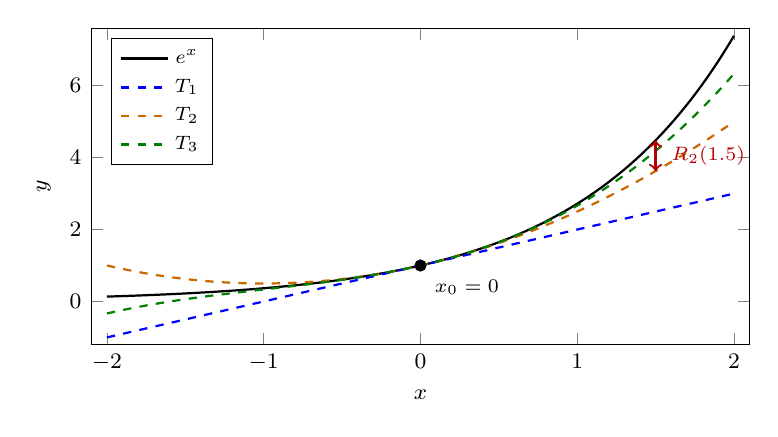
\begin{tikzpicture}
\begin{axis}[width=0.82\linewidth, height=5.6cm,
  xlabel={$x$}, ylabel={$y$},
  xmin=-2.1, xmax=2.1, ymin=-1.2, ymax=7.6,
  xtick={-2,-1,0,1,2}, ytick={0,2,4,6},
  domain=-2:2, samples=160, font=\footnotesize,
  legend pos=north west, legend style={font=\scriptsize}]
\addplot[black,thick] {exp(x)};
\addlegendentry{$e^x$}
\addplot[blue,thick,dashed] {1+x};
\addlegendentry{$T_1$}
\addplot[orange!80!black,thick,dashed] {1+x+x^2/2};
\addlegendentry{$T_2$}
\addplot[green!50!black,thick,dashed] {1+x+x^2/2+x^3/6};
\addlegendentry{$T_3$}
\draw[<->,red!70!black,thick] (axis cs:1.5,3.625) -- (axis cs:1.5,4.4817);
\node[font=\scriptsize,red!70!black,anchor=west] at (axis cs:1.54,4.05) {$R_2(1.5)$};
\addplot[only marks,mark=*,black] coordinates {(0,1)};
\node[font=\scriptsize,anchor=north west] at (axis cs:0.03,0.88) {$x_0=0$};
\end{axis}
\end{tikzpicture}\\[2pt]
{\footnotesize 图 7：$T_1,T_2,T_3$ 在 $0$ 处分别与 $e^x$ 重合到 $1,2,3$ 阶导数。竖直双箭头是 $x=1.5$ 处的余项 $R_2$；阶数越高，贴合的范围越大，但仍然是局部逼近。}
\end{center}

泰勒多项式是唯一的。若
\[
f(x)=a_0+a_1(x-x_0)+\cdots+a_n(x-x_0)^n+o\bigl((x-x_0)^n\bigr),
\]
则 $a_k=\dfrac{f^{(k)}(x_0)}{k!}$。理由很简单：先令 $x\to x_0$ 得 $a_0=f(x_0)$；减去 $a_0$，除以 $x-x_0$ 再取极限，得 $a_1=f'(x_0)$；依此类推。这条性质允许我们不去逐阶求导，而是用已知展开式做代换、相乘、相除，得到新的展开。

$x_0=0$ 时，泰勒公式叫麦克劳林公式。下面五个展开式要熟到能直接写出来。

\begin{center}
\footnotesize
\renewcommand{\arraystretch}{1.5}
\begin{tabular}{@{}l p{0.70\linewidth}@{}}
\toprule
函数 & 麦克劳林展开（带皮亚诺余项）\\
\midrule
$e^x$ & $1+x+\dfrac{x^2}{2!}+\cdots+\dfrac{x^n}{n!}+o(x^n)$\\[2pt]
$\sin x$ & $x-\dfrac{x^3}{3!}+\dfrac{x^5}{5!}-\cdots+(-1)^n\dfrac{x^{2n+1}}{(2n+1)!}+o(x^{2n+2})$\\[2pt]
$\cos x$ & $1-\dfrac{x^2}{2!}+\dfrac{x^4}{4!}-\cdots+(-1)^n\dfrac{x^{2n}}{(2n)!}+o(x^{2n+1})$\\[2pt]
$\ln(1+x)$ & $x-\dfrac{x^2}{2}+\dfrac{x^3}{3}-\cdots+(-1)^{n-1}\dfrac{x^n}{n}+o(x^n)$\\[2pt]
$(1+x)^\alpha$ & $1+\alpha x+\dfrac{\alpha(\alpha-1)}{2!}x^2+\cdots+\dfrac{\alpha(\alpha-1)\cdots(\alpha-n+1)}{n!}x^n+o(x^n)$\\
\bottomrule
\end{tabular}
\end{center}

表中 $o$ 的阶数与最后写出的项有关。写到 $x^n$，余项就是 $o(x^n)$；$\sin x$ 写到 $x^{2n+1}$，下一项是 $x^{2n+3}$，所以余项写成 $o(x^{2n+2})$ 也成立。实际计算时只要保证需要的那一阶没有丢掉即可。

\begin{center}
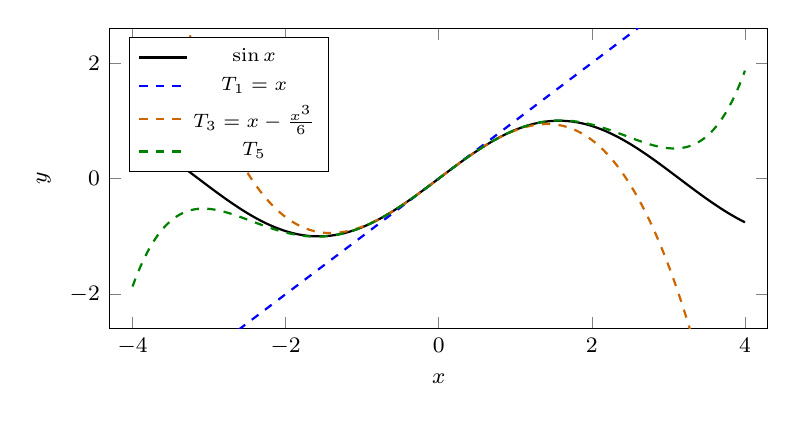
\begin{tikzpicture}
\begin{axis}[width=0.82\linewidth, height=5.4cm,
  xlabel={$x$}, ylabel={$y$},
  xmin=-4.3, xmax=4.3, ymin=-2.6, ymax=2.6,
  xtick={-4,-2,0,2,4}, ytick={-2,0,2},
  domain=-4:4, samples=240, font=\footnotesize,
  legend pos=north west, legend style={font=\scriptsize}]
\addplot[black,thick] {sin(deg(x))};
\addlegendentry{$\sin x$}
\addplot[blue,thick,dashed] {x};
\addlegendentry{$T_1=x$}
\addplot[orange!80!black,thick,dashed] {x-x^3/6};
\addlegendentry{$T_3=x-\frac{x^3}{6}$}
\addplot[green!50!black,thick,dashed] {x-x^3/6+x^5/120};
\addlegendentry{$T_5$}
\end{axis}
\end{tikzpicture}\\[2pt]
{\footnotesize 图 8：三条泰勒多项式都在 $0$ 附近贴合 $\sin x$。离开 $0$ 后，低阶的先偏离，$T_5$ 的有效范围最大。}
\end{center}

\subsection{泰勒公式的用法}

\paragraph{求极限.} 把分子分母各自展开到相同的阶，低阶项会抵消，剩下的最低阶项决定极限。例如
\[
\lim_{x\to0}\frac{e^x-1-x}{x^2}
=\lim_{x\to0}\frac{\frac{x^2}{2}+o(x^2)}{x^2}
=\frac12.
\]
这里用了 $e^x=1+x+\dfrac{x^2}{2}+o(x^2)$。如果只展开到 $x$，分子变成 $o(x)$，与分母 $x^2$ 不同阶，说明展开得不够，需要再往下一阶。再看
\[
\lim_{x\to0}\frac{\sin x-x}{x^3}
=\lim_{x\to0}\frac{-\frac{x^3}{6}+o(x^3)}{x^3}
=-\frac16.
\]
分母是 $x^3$，所以 $\sin x$ 要展开到 $x^3$。

\paragraph{判断无穷小的阶.} 从上面的计算还能读出阶数：$e^x-1-x$ 与 $\dfrac{x^2}{2}$ 等价，是二阶无穷小；$\sin x-x$ 与 $-\dfrac{x^3}{6}$ 等价，是三阶无穷小。把函数展开到首个非零项，看它是 $x$ 的几次方，就是它的阶。

\paragraph{证明不等式.} 关键是让余项的符号确定。对 $x>0$，在 $0$ 与 $x$ 之间用带拉格朗日余项的二阶泰勒公式：
\[
e^x=1+x+\frac{x^2}{2}+\frac{e^\xi}{6}x^3,\qquad \xi\in(0,x).
\]
余项为正，所以 $e^x>1+x+\dfrac{x^2}{2}$。注意 $x<0$ 时 $x^3<0$，余项为负，不等号反过来。泰勒多项式不一定总在函数上方或下方，要看 $(x-x_0)^{n+1}$ 的符号。

再比如 $0<x<\pi$ 时，
\[
\sin x=x-\frac{x^3}{6}+\frac{\sin\xi}{24}x^4,
\]
其中 $\xi\in(0,x)$，$\sin\xi>0$，所以 $\sin x>x-\dfrac{x^3}{6}$。选择展开点和阶数时，要让余项中的导数在区间上有确定的符号或界。

\paragraph{估计误差.} 若不需要知道 $\xi$，只估计误差的大小：
\[
|R_n(x)|\le \frac{M}{(n+1)!}|x-x_0|^{n+1},
\]
其中 $M$ 是 $|f^{(n+1)}|$ 在区间上的上界。例如在 $|x|\le1$ 上用 $T_2$ 近似 $e^x$，有
\[
|R_2(x)|\le\frac{e}{6}|x|^3\le\frac{e}{6}\approx0.45.
\]
实际误差通常比这个界小，但界是可以保证的。

\paragraph{判断高阶极值.} 若
\[
f'(x_0)=f''(x_0)=\cdots=f^{(n-1)}(x_0)=0,\qquad f^{(n)}(x_0)\ne0,
\]
则由带皮亚诺余项的泰勒公式，
\[
f(x)-f(x_0)=\frac{f^{(n)}(x_0)}{n!}(x-x_0)^n+o\bigl((x-x_0)^n\bigr).
\]
$x$ 足够靠近 $x_0$ 时，右端第一项决定符号。$n$ 为偶数时，$(x-x_0)^n$ 在两侧都为正，$f(x)-f(x_0)$ 两侧同号，$x_0$ 是极值点；$n$ 为奇数时，两侧异号，$x_0$ 不是极值点。符号由 $f^{(n)}(x_0)$ 决定：$n$ 偶且 $f^{(n)}(x_0)>0$ 为极小值，$f^{(n)}(x_0)<0$ 为极大值。例如 $x^4$ 在 $0$ 处四阶导数为 $24>0$，是极小值；$x^3$ 在 $0$ 处三阶导数为 $6\ne0$，$n$ 为奇数，不是极值。

\newpage
\section{习题}

\subsection{本章速览}

\begin{itemize}
\item \textbf{费马引理：}若 $f$ 在 $x_0$ 处取得极值且在该点可导，则 $f'(x_0)=0$。反之不成立：$f(x)=x^3$ 在 $x=0$ 处有 $f'(0)=0$，但 $x=0$ 不是极值点。
\item \textbf{罗尔定理：}三条件缺一不可——$f$ 在 $[a,b]$ 上连续、在 $(a,b)$ 内可导、$f(a)=f(b)$；结论是存在 $\xi\in(a,b)$ 使 $f'(\xi)=0$。只给开区间内可导而不给端点连续，结论可能失效。
\item \textbf{拉格朗日中值定理：}$f(b)-f(a)=f'(\xi)(b-a)$，$\xi\in(a,b)$。它把函数增量、自变量增量与导数联系起来，是证明不等式、判断单调性和推出“导数恒为零则函数为常数”的基本工具。
\item \textbf{柯西中值定理：}在连续、可导之外还要求 $g'(x)\neq 0$，结论为 $\frac{f(b)-f(a)}{g(b)-g(a)}=\frac{f'(\xi)}{g'(\xi)}$。取 $g(x)=x$ 即得拉格朗日中值定理。
\item \textbf{泰勒公式：}带皮亚诺余项 $o((x-x_0)^n)$ 用于求极限、判断无穷小阶数；带拉格朗日余项 $\dfrac{f^{(n+1)}(\xi)}{(n+1)!}(x-x_0)^{n+1}$ 用于不等式证明与误差估计。两种余项的多项式部分完全相同。
\item \textbf{辅助函数套路：}要证含 $f'(\xi)$ 与 $f(\xi)$ 的关系式，把结论中的 $\xi$ 换成 $x$ 看成微分方程，其解就是辅助函数。常用：$e^{g(x)}f(x)$、$x^nf(x)$、$\dfrac{f(x)}{g(x)}$、$f(x)g(x)$。
\end{itemize}

\subsection{基础过关题}

\textbf{1.} 验证函数 $f(x)=x^{3}-9x^{2}+23x-15$ 在区间 $[1,5]$ 上满足罗尔定理的条件，并求出定理结论中所有的 $\xi$。

\ifshowsolutions%
\boxed{\textbf{解}}
\textbf{思路：}先验证三个条件，再解方程 $f'(x)=0$，最后检查所得根是否落在开区间 $(1,5)$ 内。

$f$ 是多项式，在 $[1,5]$ 上连续、在 $(1,5)$ 内可导。计算端点值：
\[
f(1)=1-9+23-15=0,\qquad f(5)=125-225+115-15=0,
\]
故 $f(1)=f(5)$，罗尔定理的三个条件全部满足。

求导并因式分解：
\[
f'(x)=3x^{2}-18x+23.
\]
令 $f'(x)=0$，得
\[
x=\frac{18\pm\sqrt{324-4\cdot 3\cdot 23}}{6}
=\frac{18\pm\sqrt{48}}{6}
=3\pm\frac{2\sqrt3}{3}.
\]
其中 $3-\frac{2\sqrt3}{3}\approx 1.845$，$3+\frac{2\sqrt3}{3}\approx 4.155$，二者都落在 $(1,5)$ 内，因此都是罗尔定理中的 $\xi$。

\boxed{\textbf{答案：}\xi=3\pm\dfrac{2\sqrt3}{3}}
\else \answerarea[8] \fi%

\textbf{2.} 设 $f(x)=\ln x$。验证 $f$ 在 $[1,e]$ 上满足拉格朗日中值定理的条件，并求出定理中的 $\xi$。

\ifshowsolutions%
\boxed{\textbf{解}}
\textbf{思路：}$\ln x$ 在 $[1,e]$ 上连续、在 $(1,e)$ 内可导，直接由中值公式列方程解 $\xi$。

$f(x)=\ln x$ 在 $[1,e]$ 上连续，在 $(1,e)$ 内可导，且 $f'(x)=\dfrac1x$，条件满足。由拉格朗日中值定理，存在 $\xi\in(1,e)$ 使
\[
\frac{f(e)-f(1)}{e-1}=f'(\xi),
\]
即
\[
\frac{1-0}{e-1}=\frac1{\xi}.
\]
解得 $\xi=e-1$。由于 $e\approx 2.718$，故 $\xi=e-1\approx 1.718$，确实满足 $1<\xi<e$。

\boxed{\textbf{答案：}\xi=e-1}
\else \answerarea[8] \fi%

\textbf{3.} 设 $f(x)=\sin x$，$g(x)=\cos x$。在区间 $\left[0,\dfrac{\pi}{2}\right]$ 上验证柯西中值定理，并求出定理中的 $\xi$。

\ifshowsolutions%
\boxed{\textbf{解}}
\textbf{思路：}柯西中值定理比对值 $\dfrac{f'(\xi)}{g'(\xi)}$，先确认 $g'$ 在开区间内不为零，再解三角方程。

$f,g$ 在 $\left[0,\frac{\pi}{2}\right]$ 上连续，在 $\left(0,\frac{\pi}{2}\right)$ 内可导，且
\[
g'(x)=-\sin x\neq 0,\qquad x\in\left(0,\frac{\pi}{2}\right),
\]
条件满足。计算两端之差：
\[
f\left(\frac{\pi}{2}\right)-f(0)=1-0=1,\qquad
g\left(\frac{\pi}{2}\right)-g(0)=0-1=-1.
\]
由柯西中值定理，存在 $\xi\in\left(0,\frac{\pi}{2}\right)$ 使
\[
\frac{1}{-1}=\frac{\cos\xi}{-\sin\xi}=-\cot\xi,
\]
即 $\cot\xi=1$，从而 $\tan\xi=1$，$\xi=\dfrac{\pi}{4}$，它落在 $\left(0,\frac{\pi}{2}\right)$ 内。

\boxed{\textbf{答案：}\xi=\dfrac{\pi}{4}}
\else \answerarea[8] \fi%

\textbf{4.} 证明：当 $x>0$ 时，
\[
\frac{x}{1+x}<\ln(1+x)<x.
\]

\ifshowsolutions%
\boxed{\textbf{解}}
\textbf{思路：}把 $\ln(1+x)-\ln 1$ 写成 $x\cdot\dfrac{1}{1+\xi}$，再用 $\xi\in(0,x)$ 夹出上下界。

对 $F(t)=\ln(1+t)$ 在 $[0,x]$ 上使用拉格朗日中值定理。$F$ 在 $[0,x]$ 上连续、在 $(0,x)$ 内可导，$F'(t)=\dfrac{1}{1+t}$，故存在 $\xi\in(0,x)$ 使
\[
\ln(1+x)-\ln 1=\frac{1}{1+\xi}\,(x-0),
\]
即
\[
\ln(1+x)=\frac{x}{1+\xi}.
\]
由 $0<\xi<x$ 得 $1<1+\xi<1+x$，取倒数（各项为正）得
\[
\frac{1}{1+x}<\frac{1}{1+\xi}<1.
\]
三边同乘正数 $x$，得
\[
\frac{x}{1+x}<\frac{x}{1+\xi}<x,
\]
即 $\dfrac{x}{1+x}<\ln(1+x)<x$。

\boxed{\textbf{答案：}\text{不等式对一切 }x>0\text{ 成立}}
\else \answerarea[8] \fi%

\textbf{5.} 求极限
\[
\lim_{x\to 0}\frac{\cos x-e^{-x^{2}/2}}{x^{4}}.
\]

\ifshowsolutions%
\boxed{\textbf{解}}
\textbf{思路：}分子中两项都展开到 $x^4$ 阶，低阶项应恰好抵消，剩余的最低阶项决定极限。

由麦克劳林公式
\[
\cos x=1-\frac{x^{2}}{2}+\frac{x^{4}}{24}+o(x^{4}).
\]
对 $e^{u}=1+u+\dfrac{u^{2}}{2}+o(u^{2})$ 取 $u=-\dfrac{x^{2}}{2}$，得
\[
e^{-x^{2}/2}=1-\frac{x^{2}}{2}+\frac{1}{2}\left(-\frac{x^{2}}{2}\right)^{2}+o(x^{4})
=1-\frac{x^{2}}{2}+\frac{x^{4}}{8}+o(x^{4}).
\]
两式相减，$1$ 与 $-\dfrac{x^{2}}{2}$ 都抵消：
\[
\cos x-e^{-x^{2}/2}
=\left(\frac{1}{24}-\frac18\right)x^{4}+o(x^{4})
=-\frac{1}{12}x^{4}+o(x^{4}).
\]
于是
\[
\lim_{x\to 0}\frac{\cos x-e^{-x^{2}/2}}{x^{4}}
=\lim_{x\to 0}\frac{-\frac{1}{12}x^{4}+o(x^{4})}{x^{4}}
=-\frac{1}{12}.
\]

\boxed{\textbf{答案：}-\dfrac{1}{12}}
\else \answerarea[8] \fi%

\subsection{综合提高题}

\textbf{6.} 讨论方程 $x^{3}-3x+1=0$ 的实根个数，并指出每个根所在的区间。

\ifshowsolutions%
\boxed{\textbf{解}}
\textbf{思路：}先用导数确定单调区间与极值，结合两端极限说明“至少”有几个根；再用罗尔定理说明“至多”有几个根。

设 $f(x)=x^{3}-3x+1$，则
\[
f'(x)=3x^{2}-3=3(x-1)(x+1).
\]
$f'$ 的零点为 $x=-1$ 和 $x=1$，列表可知：$f$ 在 $(-\infty,-1)$ 上递增，在 $(-1,1)$ 上递减，在 $(1,+\infty)$ 上递增。极值为
\[
f(-1)=-1+3+1=3>0\ (\text{极大值}),\quad
f(1)=1-3+1=-1<0\ (\text{极小值}).
\]
又 $\lim\limits_{x\to-\infty}f(x)=-\infty$，$\lim\limits_{x\to+\infty}f(x)=+\infty$。

在三个单调区间上分别用零点定理：
\begin{itemize}
\item $(-\infty,-1)$：$f(-2)=-8+6+1=-1<0$，$f(-1)=3>0$，故在 $(-2,-1)$ 内有一个根，且由严格单调知只有一个；
\item $(-1,1)$：$f(-1)=3>0$，$f(1)=-1<0$，故在 $(-1,1)$ 内有一个根，且只有一个；
\item $(1,+\infty)$：$f(1)=-1<0$，$f(2)=8-6+1=3>0$，故在 $(1,2)$ 内有一个根，且只有一个。
\end{itemize}
所以至少有 $3$ 个实根。若实根多于 $3$ 个，即至少有 $4$ 个，则对 $f$ 连续使用三次罗尔定理，$f'$ 至少要有 $3$ 个零点；但 $f'=3(x-1)(x+1)$ 只有 $x=\pm1$ 两个零点，矛盾。因此恰有 $3$ 个实根。

\boxed{\textbf{答案：}\text{恰有 }3\text{ 个实根，分别在 }(-2,-1),\,(-1,1),\,(1,2)\text{ 内}}
\else \answerarea[10] \fi%

\textbf{7.} 设 $f$ 在 $[0,1]$ 上连续，在 $(0,1)$ 内可导，$f(0)=0$，且 $f'$ 在 $(0,1)$ 内严格单调递增。证明：函数
\[
g(x)=\frac{f(x)}{x}
\]
在 $(0,1)$ 内严格单调递增。

\ifshowsolutions%
\boxed{\textbf{解}}
\textbf{思路：}直接对 $g$ 求导，分子 $xf'(x)-f(x)$ 可以借助中值定理写成 $x\bigl(f'(x)-f'(\xi)\bigr)$，再用 $f'$ 的单调性定号。

对 $x\in(0,1)$，
\[
g'(x)=\frac{xf'(x)-f(x)}{x^{2}}.
\]
因为 $f$ 在 $[0,x]$ 上连续、在 $(0,x)$ 内可导，由拉格朗日中值定理，存在 $\xi\in(0,x)$ 使
\[
f(x)-f(0)=f'(\xi)(x-0),
\]
结合 $f(0)=0$ 得 $f(x)=xf'(\xi)$。代入分子：
\[
xf'(x)-f(x)=xf'(x)-xf'(\xi)=x\bigl[f'(x)-f'(\xi)\bigr].
\]
由于 $0<\xi<x<1$ 且 $f'$ 在 $(0,1)$ 内严格单调递增，故 $f'(x)>f'(\xi)$，从而
\[
xf'(x)-f(x)>0.
\]
于是 $g'(x)>0$ 对一切 $x\in(0,1)$ 成立，$g$ 在 $(0,1)$ 内严格单调递增。

\boxed{\textbf{答案：}\text{证明如上。}}
\else \answerarea[10] \fi%

\textbf{8.} 证明：当 $x>0$ 时，
\[
\ln(1+x)<x-\frac{x^{2}}{2}+\frac{x^{3}}{3}.
\]

\ifshowsolutions%
\boxed{\textbf{解}}
\textbf{思路：}右端正是 $\ln(1+x)$ 的三阶泰勒多项式。把函数在 $0$ 处展开到三阶，用拉格朗日余项的符号判断大小。

设 $f(t)=\ln(1+t)$，则
\[
f(0)=0,\quad f'(t)=\frac{1}{1+t},\quad f''(t)=-\frac{1}{(1+t)^{2}},
\]
\[
f'''(t)=\frac{2}{(1+t)^{3}},\quad f^{(4)}(t)=-\frac{6}{(1+t)^{4}}.
\]
于是 $f'(0)=1$，$f''(0)=-1$，$f'''(0)=2$。在 $[0,x]$ 上使用带拉格朗日余项的三阶泰勒公式，存在 $\xi\in(0,x)$ 使
\[
f(x)=f(0)+f'(0)x+\frac{f''(0)}{2!}x^{2}+\frac{f'''(0)}{3!}x^{3}
+\frac{f^{(4)}(\xi)}{4!}x^{4}.
\]
代入各导数：
\[
\ln(1+x)=x-\frac{x^{2}}{2}+\frac{x^{3}}{3}
-\frac{6}{(1+\xi)^{4}}\cdot\frac{x^{4}}{24}
=x-\frac{x^{2}}{2}+\frac{x^{3}}{3}-\frac{x^{4}}{4(1+\xi)^{4}}.
\]
因为 $x>0$，$\xi\in(0,x)$，所以 $\dfrac{x^{4}}{4(1+\xi)^{4}}>0$，从而
\[
\ln(1+x)<x-\frac{x^{2}}{2}+\frac{x^{3}}{3}.
\]

\boxed{\textbf{答案：}\text{证明如上。}}
\else \answerarea[10] \fi%

\textbf{9.} 设 $f$ 在 $[0,1]$ 上具有连续的二阶导数，$f(0)=f(1)=0$，且 $|f''(x)|\le M$（$x\in[0,1]$）。证明：对任意 $x\in[0,1]$，
\[
|f'(x)|\le\frac{M}{2}.
\]

\ifshowsolutions%
\boxed{\textbf{解}}
\textbf{思路：}在任意点 $x$ 处向两个端点各写一次带拉格朗日余项的一阶泰勒公式，两式相减消去 $f(x)$，只剩 $f'(x)$ 与两个二阶导数。

先设 $x\in(0,1)$。分别以 $x$ 为展开点，把 $f(0)$、$f(1)$ 展开：
\[
0=f(0)=f(x)+f'(x)(0-x)+\frac{f''(\xi_1)}{2}(0-x)^{2},
\]
\[
0=f(1)=f(x)+f'(x)(1-x)+\frac{f''(\xi_2)}{2}(1-x)^{2},
\]
其中 $\xi_1\in(0,x)$，$\xi_2\in(x,1)$。即
\[
0=f(x)-xf'(x)+\frac{x^{2}}{2}f''(\xi_1),\tag{1}
\]
\[
0=f(x)+(1-x)f'(x)+\frac{(1-x)^{2}}{2}f''(\xi_2).\tag{2}
\]
$(1)-(2)$ 消去 $f(x)$：
\[
0=-f'(x)+\frac{x^{2}}{2}f''(\xi_1)-\frac{(1-x)^{2}}{2}f''(\xi_2),
\]
故
\[
f'(x)=\frac{x^{2}}{2}f''(\xi_1)-\frac{(1-x)^{2}}{2}f''(\xi_2).
\]
取绝对值并用 $|f''|\le M$：
\[
|f'(x)|\le\frac{M}{2}\bigl[x^{2}+(1-x)^{2}\bigr].
\]
而
\[
x^{2}+(1-x)^{2}=2\left(x-\frac12\right)^{2}+\frac12\le 1,\qquad x\in[0,1],
\]
所以 $|f'(x)|\le\dfrac{M}{2}$。

再补端点。对 $x=0$，在 $[0,1]$ 上把 $f(1)$ 在 $0$ 处展开：
\[
0=f(1)=f(0)+f'(0)\cdot 1+\frac{f''(\xi)}{2}\cdot 1^{2}
=f'(0)+\frac{f''(\xi)}{2},
\]
故 $|f'(0)|=\dfrac{|f''(\xi)|}{2}\le\dfrac{M}{2}$。同理，把 $f(0)$ 在 $1$ 处展开可得 $|f'(1)|\le\dfrac{M}{2}$。

最后说明系数 $\dfrac12$ 不可改进：取 $f(x)=\dfrac{M}{2}x(1-x)$，则 $f(0)=f(1)=0$，$f''(x)=-M$ 满足 $|f''|\le M$，而 $f'(0)=\dfrac{M}{2}$，恰好取到等号。

\boxed{\textbf{答案：}|f'(x)|\le\dfrac{M}{2}\text{，且 }\dfrac12\text{ 不可改进}}
\else \answerarea[10] \fi%

\subsection{真题风格与综合训练}

\textbf{10.}（单项选择题）下列命题中正确的是

\begin{center}
\begin{tabular}{p{0.46\linewidth}p{0.46\linewidth}}
(A) 若 $f$ 在 $x_0$ 处取得极值，则 $f'(x_0)=0$； & (B) 若 $f$ 在 $[a,b]$ 上连续、在 $(a,b)$ 内可导且 $f(a)=f(b)$，则存在 $\xi\in(a,b)$ 使 $f'(\xi)=0$；\\[4pt]
(C) 若 $f'(\xi)=0$，则 $\xi$ 必为 $f$ 的极值点； & (D) 若 $f$ 在 $[a,b]$ 上连续、在 $(a,b)$ 内可导且只有一个驻点，则该驻点必为极值点。
\end{tabular}
\end{center}

\ifshowsolutions%
\boxed{\textbf{解}}
\textbf{思路：}逐项检查定理条件，凡缺少“可导”“连续”或把必要条件当充分条件者均可构造反例。

(A) 错。费马引理还要求 $f$ 在 $x_0$ 处可导。反例：$f(x)=|x|$ 在 $x=0$ 处取得极小值，但 $f'(0)$ 不存在。

(B) 对。这正是罗尔定理，三个条件齐备。

(C) 错。驻点未必是极值点。反例：$f(x)=x^{3}$，$f'(0)=0$，但 $f$ 在 $0$ 两侧都递增，$x=0$ 不是极值点。

(D) 错。反例：$f(x)=x^{3}$ 在 $[-1,1]$ 上只有一个驻点 $x=0$，但 $x=0$ 不是极值点。

\boxed{\textbf{答案：}(B)}
\else \answerarea[8] \fi%

\textbf{11.}（填空题）当 $x\to 0$ 时，$\ln(1+x)-x+\dfrac{x^{2}}{2}$ 与 $ax^{k}$ 是等价无穷小，则 $a=\underline{\qquad}$，$k=\underline{\qquad}$。

\ifshowsolutions%
\boxed{\textbf{解}}
\textbf{思路：}把 $\ln(1+x)$ 展开到首个未被抵消的阶，比较系数即可。

由麦克劳林公式
\[
\ln(1+x)=x-\frac{x^{2}}{2}+\frac{x^{3}}{3}+o(x^{3}),
\]
所以
\[
\ln(1+x)-x+\frac{x^{2}}{2}=\frac{x^{3}}{3}+o(x^{3}).
\]
因此它与 $\dfrac13x^{3}$ 等价，即 $a=\dfrac13$，$k=3$。

\boxed{\textbf{答案：}a=\dfrac13,\ k=3}
\else \answerarea[3] \fi%

\textbf{12.}（解答题）设 $f$ 在 $[0,1]$ 上具有连续的二阶导数，$f(0)=f(1)=0$，$f'(0)=1$。证明：存在 $\xi\in(0,1)$，使得
\[
f''(\xi)=-2.
\]

\ifshowsolutions%
\boxed{\textbf{解}}
\textbf{思路：}要证的式子等价于某个辅助函数的二阶导数为零。把 $-2$ 移过去看成 $f''+2=0$，积分两次得辅助函数 $g(x)=f(x)+x^{2}-x$。

令
\[
g(x)=f(x)+x^{2}-x=f(x)-x(1-x).
\]
则 $g$ 在 $[0,1]$ 上具有连续的二阶导数，且
\[
g(0)=f(0)+0-0=0,\qquad g(1)=f(1)+1-1=0.
\]
由罗尔定理，存在 $c\in(0,1)$ 使
\[
g'(c)=0.
\]
另一方面
\[
g'(x)=f'(x)+2x-1,\qquad g'(0)=f'(0)-1=1-1=0.
\]
于是 $g'$ 在 $[0,c]$ 上连续、在 $(0,c)$ 内可导，且 $g'(0)=g'(c)=0$。再次使用罗尔定理，存在 $\xi\in(0,c)\subset(0,1)$ 使
\[
g''(\xi)=0.
\]
而 $g''(x)=f''(x)+2$，故 $f''(\xi)+2=0$，即 $f''(\xi)=-2$。

\boxed{\textbf{答案：}\text{证明如上。}}
\else \answerarea[10] \fi%

